\documentclass[10pt,a4paper,final]{article}
%
\usepackage[utf8x]{inputenc}
\usepackage{ucs}
\usepackage{amsmath}
\usepackage{geometry}
\usepackage{anysize} % Soporte para el comando \marginsize
\usepackage{graphicx}
\usepackage{amsfonts}
\usepackage{amssymb}
\usepackage[spanish]{babel}
%%%%%%%%%%%%%%%%%%%%%%%%%%%%%%%%%%%%%%%%%%%%%%%%%
%%%%%%%%%%%%%%%%%%%%%%%%%%%%%%%%%%%%%%%%%%%%%%%%%
%%%%%%%%%%%%%%%%%%%%%%%%%%%%%%%%%%%%%%%%%%%%%%%%%
\marginsize{2cm}{2cm}{1.5cm}{1.5cm}
%
\begin{document}
\title{Calculo de descensos en un campo de bombeo en medios porosos}
\author{Christian N. Pfarher, Juan Pablo Garbarino, Marina Castro\\
\textit{Trabajo práctico final de ``Métodos numéricos y simulación'', II-FICH-UNL.}}
\markboth{Método numérico y simulación: TRABAJO FINAL}{}
\date{\today}
\maketitle
%%%%%%%%%%%%%%%%%%%%%%%%%%%%%%%%%%%%%%%%%%%%%%%%%%%%%%%%%%%%%%%%%%%%%%%%%%%%%%%%%%%%%%%%%%%%%%%%%%
%%%%%%%%%%%%%%%%%%%%%%%%%%%%%%%%%%%%%%%%%%%%%%%%%%%%%%%%%%%%%%%%%%%%%%%%%%%%%%%%%%%%%%%%%%%%%%%%%%
%%%%%%%%%%%%%%%%%%%%%%%%%%%%%%%%%%%%%%%%%%%%%%%%%%%%%%%%%%%%%%%%%%%%%%%%%%%%%%%%%%%%%%%%%%%%%%%%%%
\newpage
\tableofcontents
%%%%%%%%%%%%%%%%%%%%%%%%%%%%%%%%%%%%%%%%%%%%%%%%%%%%%%%%%%%%%%%%%%%%%%%%%%%%%%%%%%%%%%%%%%%%%%%%%%
%%%%%%%%%%%%%%%%%%%%%%%%%%%%%%%%%%%%%%%%%%%%%%%%%%%%%%%%%%%%%%%%%%%%%%%%%%%%%%%%%%%%%%%%%%%%%%%%%%
%%%%%%%%%%%%%%%%%%%%%%%%%%%%%%%%%%%%%%%%%%%%%%%%%%%%%%%%%%%%%%%%%%%%%%%%%%%%%%%%%%%%%%%%%%%%%%%%%%
\newpage
%%%%%%%%%%%%%%%%%%%%%%%%%%%%%%%%%%%%%%%%%%%%%%%%%%%%%%%%%%%%%%%%%%%%%%%%%%%%%%%%%%%%%%%%%%%%%%%%%%
%%%%%%%%%%%%%%%%%%%%%%%%%%%%%%%%%%%%%%%%%%%%%%%%%%%%%%%%%%%%%%%%%%%%%%%%%%%%%%%%%%%%%%%%%%%%%%%%%%
%%%%%%%%%%%%%%%%%%%%%%%%%%%%%%%%%%%%%%%%%%%%%%%%%%%%%%%%%%%%%%%%%%%%%%%%%%%%%%%%%%%%%%%%%%%%%%%%%%
\section{Introducción}
En el presente trabajo, se presentan los resultados de la simulación de un campo de bombeo en medios porosos. El campo
consta de 2 pozos de bombeo de agua que funcionan por 15 horas seguidas. 

Para la realización del trabajo se utilizó el software de pre y pos proceso GiD \footnote{http://gid.cimne.upc.es/}. Mediante el mismo, se utilizó el \emph{módulo de pre-proceso} para la carga de los datos del problema, mientras que para
la simulación se utilizó Tdyn \footnote{es un entorno tridimensional de análisis fluidodinámico (CFD) y multifísica basado en el método de los elementos finitos estabilizado}(\emph{módulo de post-proceso}).
%%%%%%%%%%%%%%%%%%%%%%%%%%%%%%%%%%%%%%%%%%%%%%%%%%%%%%%%%%%%%%%%%%%%%%%%%%%%%%%%%%%%%%%%%%%%%%%%%%
%%%%%%%%%%%%%%%%%%%%%%%%%%%%%%%%%%%%%%%%%%%%%%%%%%%%%%%%%%%%%%%%%%%%%%%%%%%%%%%%%%%%%%%%%%%%%%%%%%
%%%%%%%%%%%%%%%%%%%%%%%%%%%%%%%%%%%%%%%%%%%%%%%%%%%%%%%%%%%%%%%%%%%%%%%%%%%%%%%%%%%%%%%%%%%%%%%%%%
\section{Objetivos}
El objetivo de este trabajo, consiste en la simulación de lineas de corrientes y equipotenciales en un campo de bombeo (medio poroso) con 2 bombas de extracción de agua en un acuífero libre (no confinado), homogéneo e isótropo.

%%%%%%%%%%%%%%%%%%%%%%%%%%%%%%%%%%%%%%%%%%%%%%%%%%%%%%%%%%%%%%%%%%%%%%%%%%%%%%%%%%%%%%%%%%%%%%%%%%
%%%%%%%%%%%%%%%%%%%%%%%%%%%%%%%%%%%%%%%%%%%%%%%%%%%%%%%%%%%%%%%%%%%%%%%%%%%%%%%%%%%%%%%%%%%%%%%%%%
%%%%%%%%%%%%%%%%%%%%%%%%%%%%%%%%%%%%%%%%%%%%%%%%%%%%%%%%%%%%%%%%%%%%%%%%%%%%%%%%%%%%%%%%%%%%%%%%%%
\section{Base Teórica}
básicamente es la ecuación de poisson con k
representado la permeabilidad.
%%%%%%%%%%%%%%%%%%%%%%%%%%%%%%%%%%%%%%%%%%%%%%%%%%%%%%%%%%%%%%%%%%%%%%%%%%%%%%%%%%%%%%%%%%%%%%%%%%%
\subsection{Modelo matemático o fisico.. ver}
describir mod mate.
 son las ecuaciones matemáticas, en nuestro caso las
ecuaciones de navier stokes\\
paredes de los costados:
	el flujo se deberia poder mover libremente... de las ecuaciones de navier stoke	(tiene como variable la velocidad (vector) y la presion (escalar)).

%%%%%%%%%%%%%%%%%%%%%%%%%%%%%%%%%%%%%%%%%%%%%%%%%%%%%%%%%%%%%%%%%%%%%%%%%%%%%%%%%%%%%%%%%%%%%%%%%%%
\subsection{Modelo numérico}
describir mod num.
tdyn resuelve en el espacio por el método de
elementos finitos y 
temporalmente hay que fijarse que opción está
tildada. *************************************************ver*******************************************
%%%%%%%%%%%%%%%%%%%%%%%%%%%%%%%%%%%%%%%%%%%%%%%%%%%%%%%%%%%%%%%%%%%%%%%%%%%%%%%%%%%%%%%%%%%%%%%%%%
%%%%%%%%%%%%%%%%%%%%%%%%%%%%%%%%%%%%%%%%%%%%%%%%%%%%%%%%%%%%%%%%%%%%%%%%%%%%%%%%%%%%%%%%%%%%%%%%%%
%%%%%%%%%%%%%%%%%%%%%%%%%%%%%%%%%%%%%%%%%%%%%%%%%%%%%%%%%%%%%%%%%%%%%%%%%%%%%%%%%%%%%%%%%%%%%%%%%%
\section{Desarrollo}
%%%%%%%%%%%%%%%%%%%%%%%%%%%%%%%%%%%%%%%%%%%%%%%%%%%%%%%%%%%%%%%%%%%%%%%%%%%%%%%%%%%%%%%%%%%%%%%%%%
\subsection{Datos del problema}
Los datos que se pudieron obtener del problema son:
\begin{itemize}
	\item Discretización del área a modelar:	
	\begin{itemize}
		\item Dominio: $x=1000 ~m.$, $y=1000 ~m.$
		\item Acuífero libre, homogéneo e isótropo $(K_x = K_y = K_z)$
		\item Espesor del acuífero: $20 ~m.$*
	\end{itemize}
	%
	\item Ubicación de los Pozos de bombeo:
	\begin{itemize}
		\item Pozo Bombeo 1: $x=150~m.$, $y=650 ~m.$
		\item Pozo Bombeo 2: $x=750~m.$, $y=250 ~m.$
	\end{itemize}
	%
	\item Caudal de bombeo:
	\begin{itemize}
		\item Pozo Bombeo 1: $60~m³/h$
		\item Pozo Bombeo 2: $40~m³/h$
		%\item[] Ambos posos trabajan 15 horas por día
	\end{itemize}
	\item Filtro: Tramo filtrante de $15~m.$ de longitud*
	\item Transmisividad: $600~m²/d$\\
\begin{LARGE}
Coef de trasmisividad: cuanto mas chiquito es mas lento se mueve el agua en el suelo.ver!! \\
\end{LARGE}	
	\item Coeficiente de almacenamiento: $5*10⁻²$ \begin{LARGE}
	creo que este no lo usamos... ver
	\end{LARGE}
	\item Porosidad efectiva: $5*10⁻²$
\end{itemize}
* Debido a problemas que se explican en el desarrollo del presente trabajo hay que aclarar que tanto el tramo filtrante como el espesor del acuífero se aumentó en un factor de 10, es decir los valores finales fueron de $150 m.$ y $200 m.$ respectivamente.\\
También hay que aclarar que nos encontramos en presencia de suelo saturado, esto es.....ver!\\
Caudal= velocidad por area ---ver aca lo de las velocidades para que de... Q=velocidad/area\\
el diametro que le pusimos  a los posos fue de 0.5m...---esto posta...

%%%%%%%%%%%%%%%%%%%%%%%%%%%%%%%%%%%%%%%%%%%%%%%%%%%%%%%%%%%%%%%%%%%%%%%%%%%%%%%%%%%%%%%%%%%%%%%%%%%
\subsection{Definición de Geometría}
Para la geometría en tres dimensiones se tiene los siguientes datos:
En las figuras \ref{cotas_superiores_generalesXY}, \ref{cotas_superiores_detallesXY} y \ref{cotas_grales_YZ} se pueden observar
las dimensiones de las geometrías según los datos del problema. Hay que aclarar aquí que el cuadrado de $300~m.~x~300~m.$ que se visualiza
en la figura \ref{cotas_superiores_detallesXY} como el rectángulo de $400~m.~x~300~m.$ en la misma figura, solo fueron dibujados con el
objetivo, de a posteriori, realizar un refinamiento del dominio en la zona que más intereza visualizar.\\
\begin{itemize}
\item Número de puntos: 33
\item Número de lineas: 52
\item Número de superficies: 28
\item Número de volumenes: 3
\end{itemize}
***************************
aclarara aca lo de los redimensioneamientos y demas...
***************************
\begin{figure}[tbhp]
\centerline{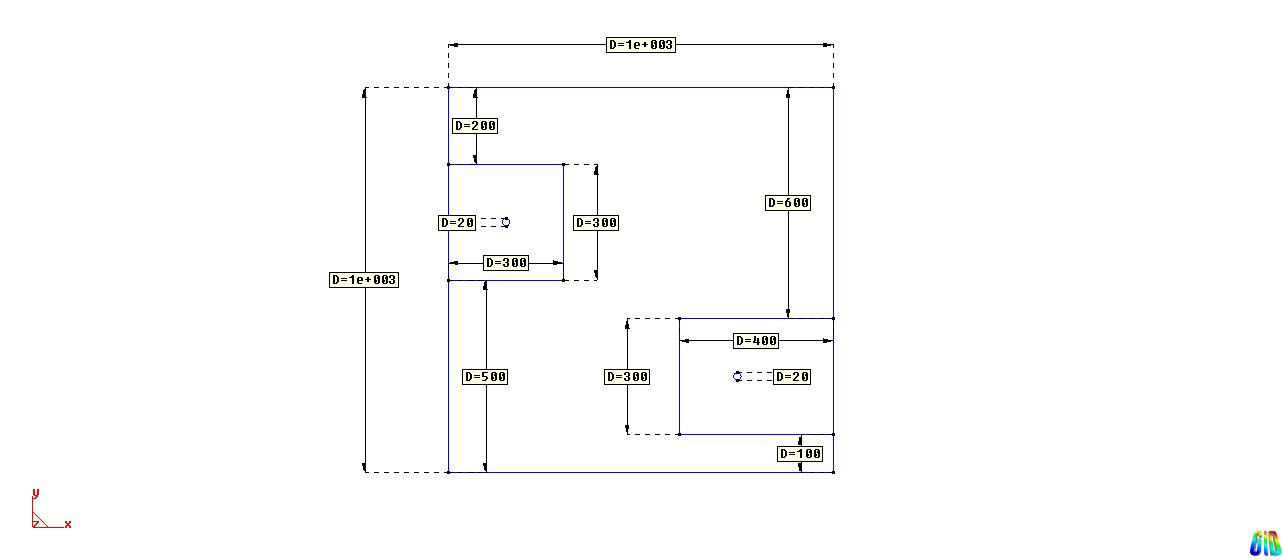
\includegraphics[scale=0.75]{img/cotas_superiores_generalesXY}}
\caption{Vista General de las cotas en el Plano XY}
\label{cotas_superiores_generalesXY}
\end{figure}

%
\begin{figure}[tbhp]
\centerline{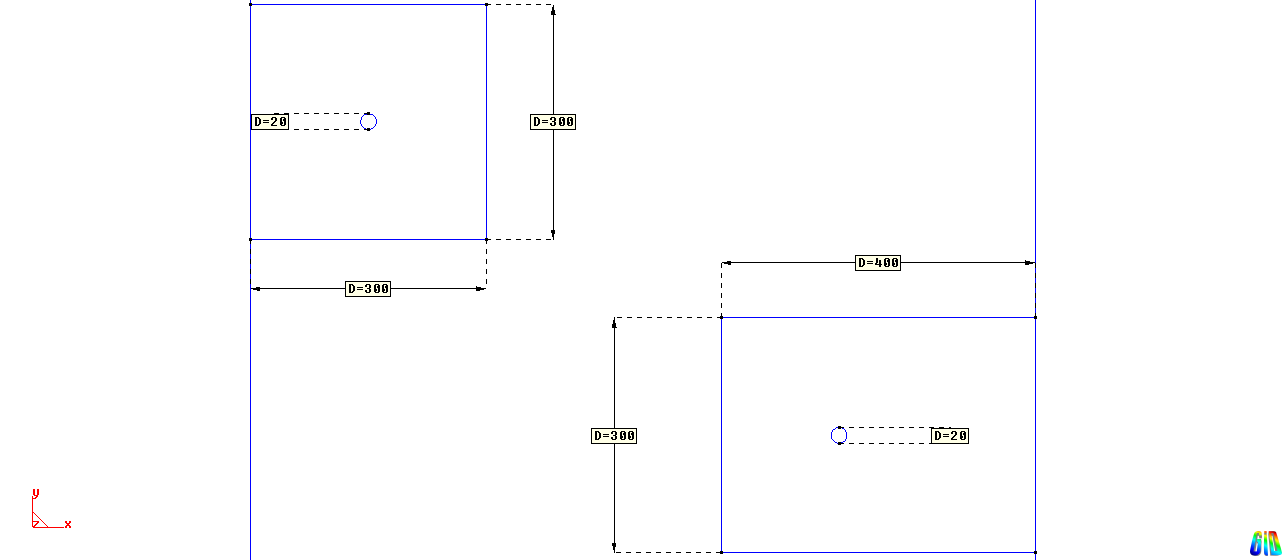
\includegraphics[scale=0.75]{img/cotas_superiores_detallesXY}}
\caption{Vista en detalle (pozos) de las cotas en el Plano XY}
\label{cotas_superiores_detallesXY}
\end{figure}
%

%
\begin{figure}[tbhp]
\centerline{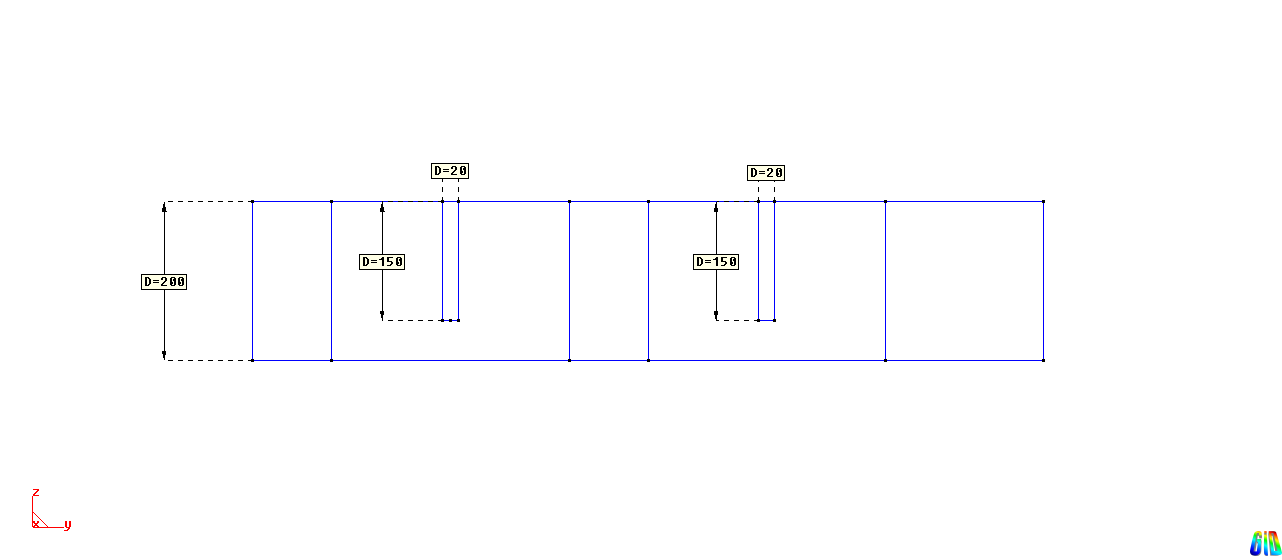
\includegraphics[scale=0.75]{img/cotas_grales_YZ}}
\caption{Vista en de las cotas en el plano YZ}
\label{cotas_grales_YZ}
\end{figure}
%
En la figura \ref{superficies_y_volumenes} se pueden observar las generaciones de las superficies (color magenta) y volúmenes (color cyan)
de la geometría.
%
\begin{figure}[tbhp]
\centerline{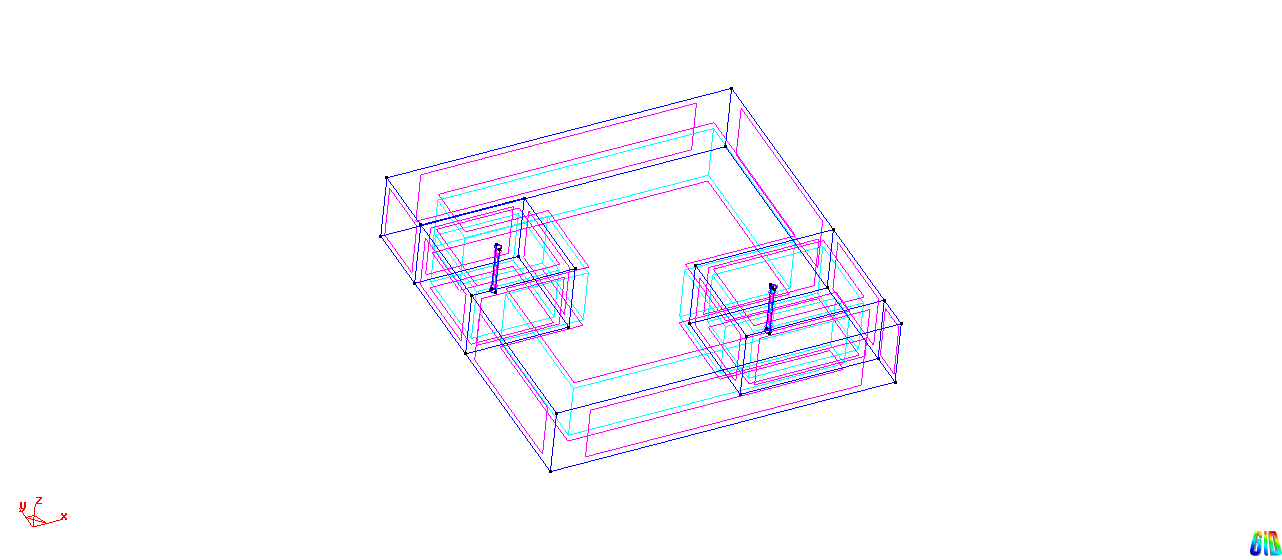
\includegraphics[scale=0.75]{img/superficies_y_volumenes}}
\caption{Superficies y Volúmenes de la Geometría}
\label{superficies_y_volumenes}
\end{figure}
%
%%%%%%%%%%%%%%%%%%%%%%%%%%%%%%%%%%%%%%%%%%%%%%%%%%%%%%%%%%%%%%%%%%%%%%%%%%%%%%%%%%%%%%%%%%%%%%%%%%%
\subsection{Propiedades del medio y de los materiales}
A partir de los datos del problema se tuvieron que realizar conversiones de unidades y el cálculo de diferentes valores para ser ingresados en el programa GID para definir los parámetros del modelo.
%%%%%%%%%%%%%%%%%%%%%%%%%%%%%%
\subsubsection{Material Suelo}
En la pestaña ransol de la ventana de materiales de fluidos para el material suelo de  se introdujeron los siguientes valores:
\begin{itemize}
\item Modelo de Fluido: incompresible
\item Densidad: $999.7~Kg/m^3$ (agua a $10° C$) \footnote{ según datos obtenidos de Tabla-libro ...}
\item Viscosidad: $0.001307~Pa.s$ (agua a $10° C$)\footnote{ según datos obtenidos de Tabla-libro ...}
\item Resistencia de la Ley de Darcy:
quizas explicar que corno y como se haya este coeficiente de 0.0000017 y que representa la ley de darcy.. porosidad del suelo...\\
	k = conductividad 1\/ m \^2 o 1 \/ darcy\\
silvina: Ley de resistencia de darcy: es la ley que habla de la velocidad que tiene el agua para moverse dentro del medio poroso. Hay 6 valores porque este coef puede ser homogeneo en todo el suelo, esto se llama suelo isotropico, es el que tiene el mismo coef de trasmisividad en todos los sentidos: x,y,z. Cuando el suelo tiene distinto coef se usa toda la matriz que es lo real y lo normal. A los fines del cálculo lo usamos como isotropico, entonces solo completamos la diag principal y con el mismo valor (hay que ver el tema de la unidad, porque esta distinta a los datos). 
\begin{equation}
\begin{pmatrix}{}
0.0000017 & 0.0 & 0.0 \\ 
0.0 & 0.0000017 & 0.0 \\ 
0.0 & 0.0 & 0.0000017
\end{pmatrix} 1/m²
\label{matrizdarcys}
\end{equation}
Debido a que se está en presencia de un acuífero isótropo, en (\ref{matrizdarcys}) se puede observar que sólo la diagonal principal de la matriz tiene valores diferentes de cero.
\end{itemize}
En la figura \ref{datos_materiales_suelo_vista} se puede observar la asignación del material definido a la parte del dominio correspondiente.

\begin{figure}[tbhp]
\centerline{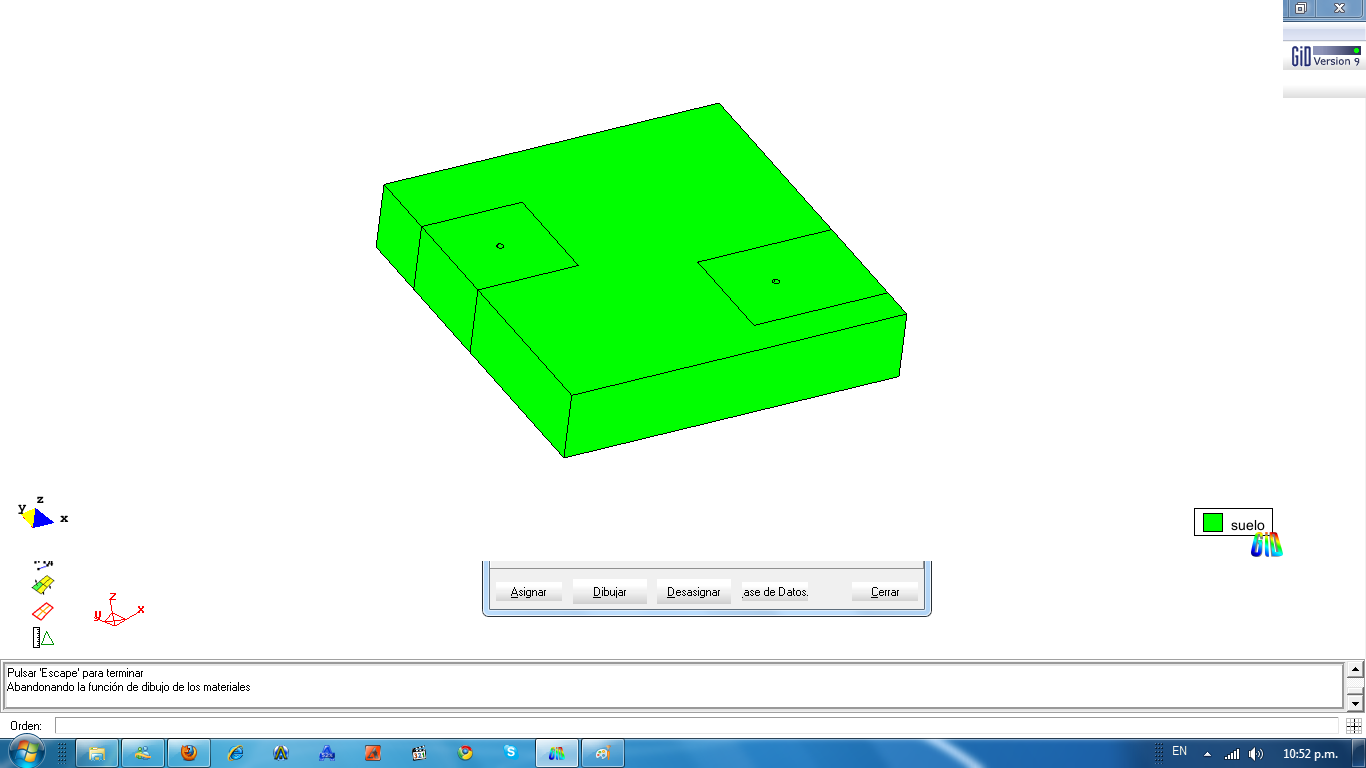
\includegraphics[scale=0.75]{img/datos_materiales_suelo_vista}}
\caption{Material Suelo asignado a la geometría}
\label{datos_materiales_suelo_vista}
\end{figure}

Características de Fluido: Flujo laminar, se comporta como viscoso por la velocidad lenta. \begin{LARGE}
que onda esto????
\end{LARGE} 
%%%%%%%%%%%%%%%%%%%%%%%%%%%%%%%
\subsubsection{Material Wall o Pared}
En la ventana de contornos fluidos se asigno a las paredes de ambos pozos el contorno definido por defecto Wall. El tipo de contorno seleccionado fue el \emph{V fixWall} con el ángulo por defecto de $60°$. Este es el modelo elegido en Tdyn para simular el comportamiento del flujo en las paredes del dominio. Básicamente, impone que la velocidad en las superficies asignadas será nula, modelando así la pared del pozo por la que no existe penetración de agua hacia el interior del pozo. En la figura \ref{datos_contornos_fluidos_vista} se puede observar el material asignado a ambos pozos.
\begin{figure}[tbhp]
\centerline{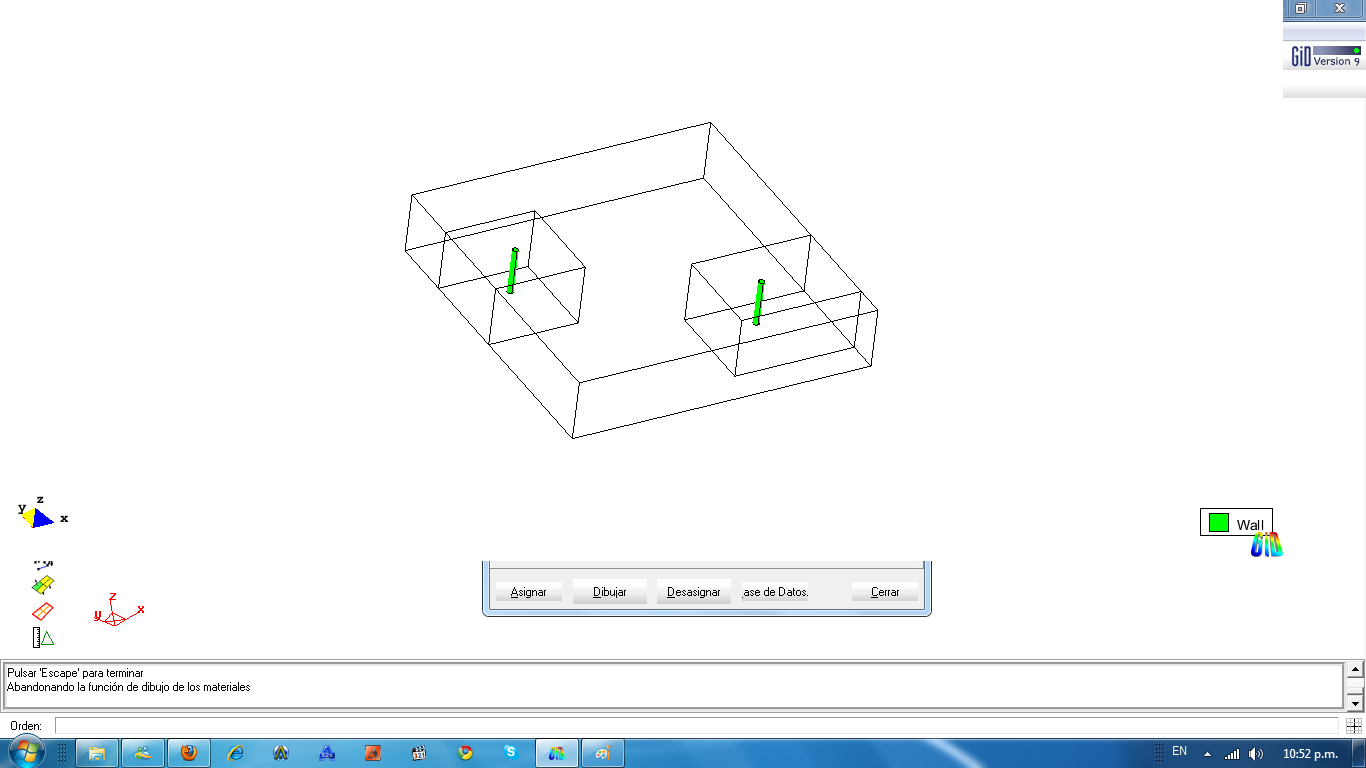
\includegraphics[scale=0.75]{img/datos_contornos_fluidos_vista}}
\caption{Material Wall o Pared asignado a la geometría}
\label{datos_contornos_fluidos_vista}
\end{figure}
%%%%%%%%%%%%%%%%%%%%%%%%%%%%%%%%%%%%%%%%%%%%%%%%%%%%%%%%%%%%%%%%%%%%%%%%%%%%%%%%%%%%%%%%%%%%%%%%%%%
\subsection{Condiciones de borde}
Para fijar las condiciones de borde, se procedió mediante el menú datos -> condiciones -> ransol. Luego se selecciono la opción de asignación de propiedades a superficies y se procedió a fijar las diferentes condiciones:
\begin{figure}[tbhp]
\centerline{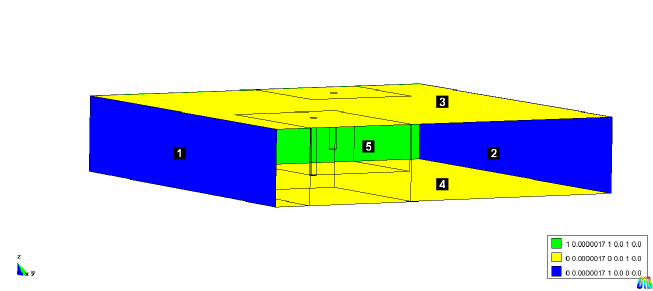
\includegraphics[scale=0.75]{img/datos_condiciones_ransol_fijar_velocidadinterno_leyendas}}
\caption{Velocidades Fijas}
\label{datos_condiciones_ransol_fijar_velocidadinterno_leyendas}
\end{figure}
%%%%%%%%%%%%%%%%%%%%%%%%%%%%%%
\subsubsection*{Fijar Velocidad}
Como se puede ver en la figura \ref{datos_condiciones_ransol_fijar_velocidadinterno_leyendas} las condiciones asignadas a cada una de las superficies enumeradas son las siguientes:

\begin{enumerate}

\item Superficie 1 y 2:

\begin{eqnarray*}
V_x&=&0.0000017~[m/s]\\
Fija~V_y&=&0.0~[m/s]\\
V_z&=&0.0~[m/s]
\end{eqnarray*}
Observar, que en las superficies 1 y 2 se fija la velocidad $V_y$ a $0$, esto se hace con el objetivo de impedir que el fluido escape del dominio (impermeabilidad de las paredes laterales). En la dirección de $x$ y $y$ el movimiento es libre.

\item Superficie 3 y 4:

\begin{eqnarray*}
V_x&=&0.0000017~[m/s]\\
V_y&=&0.0~[m/s]\\
Fija~V_z&=&0.0~[m/s]
\end{eqnarray*}

Observar, que en estas superficies se fija la velocidad $V_z$ a $0$ (para representar la impermeabilidad de la superficie superior e inferior del campo). En las direcciones de $x$ y $y$ el movimiento es libre.

\item Superficie 5:

\begin{eqnarray*}
Fija~V_x&=&0.0000017~[m/s]\\
Fija~V_y&=&0.0~[m/s]\\
Fija~V_z&=&0.0~[m/s]\\
\end{eqnarray*}

Se puede observar que en esta superficie, se fijan las velocidades en las 3 direcciones, $x$, $y$ y $z$. Esto modela la entrada de agua que se desplaza en una sola dirección ($x$). Además ese desplazamiento es a la misma velocidad con el que se determino la constante de permeabilidad $k$ de la \emph{Ley de Darcy}.

\end{enumerate}
%%%%%%%%%%%%%%%%%%%%%%%%%%%%%%
\subsubsection*{Fijar Presión}
En la figura \ref{datos_condiciones_ransol_presion} se puede observar que se fijó un valor de referencia para la presión en la superficie del extremo final de salida del campo con valor igual a $0.0~Pa$. Esto significa que los resultados que obtendremos para la presión serán relativos a esta condición.

\begin{figure}[tbhp]
\centerline{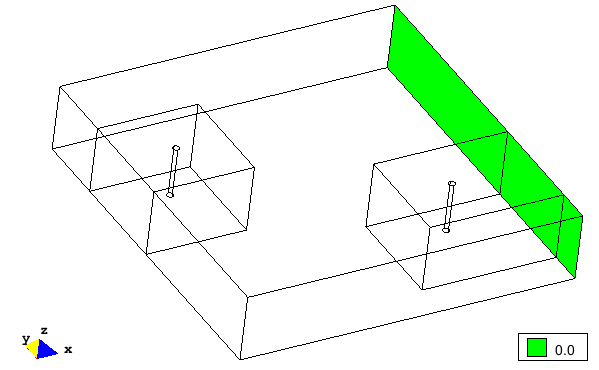
\includegraphics[scale=0.75]{img/datos_condiciones_ransol_presion}}
\caption{Condición fija de presión}
\label{datos_condiciones_ransol_presion}
\end{figure}
%%%%%%%%%%%%%%%%%%%%%%%%%%%%%%
\subsubsection*{Campo de Velocidad}
En los softwares específicos de hidrogeología, fijate que aca tenes el esquema de calculo que es una malla muy guresa en dos dimensiones, que te va a dar isocurvas de niveles. Se va a ver como esto va bombeando y ese nivel de agua cerca de la bomba va ir deprimiendose formando el cono de desenso. Eso, asi de esa forma aca no lo vamos a poder hacer, porque para poder hacer eso en 3D (en 2D si se puede) tenes que tener un soft que distinga entre suelo no saturado y suelo saturado. En el suelo saturado las ecs de gobierno son distintas a las del no saturado. El soft que tenemos solamente tiene las ecs de gob del suelo saturado, el no saturado tiene un modelo mucho mas complejo, en realidad estos modelos son bidimensionales porque no calculan el flujo en suelo saturado, lo que calculan seria la curva, la interfaz, seria la sup que los separa, nada mas, sería la ubicación de esa sup que distingue zona saturada de la no saturada. que tiene ecuaciones simples, pero no calcula detalles del flujo, este modelo calcula el flujo en suelo saturado. 
Se coincidiera que se esta en presencia de un estrato de suleo saturado (esto es saturado de agua). 
Vamos a tener lineas equipotenciales (unen lineas de igual potencial hidráulico) las cuales son perpendiculares a las lineas del flujo y serian valores de presión que ejerce el agua sobre el suelo. Esas líneas equipotenciales van a ser equivalentes en interpretacion a las lineas de superficie que se calculan tradicionalmente en hidrologia.
----------------------------
%%%%%%%%%%%%%%%%%%%%%%%%%%%%%%%%%%%%%%%%%%%%%%%%%%%%%%%%%%%%%%%%%%%%%%%%%%%%%%%%%%%%%%%%%%%%%%%%%%%
\subsection{Mallado}
Para el mallado, se asignaron diferentes tamaños a las superficies debido a que se deseó obtener un mayor detalle en las cercanías de ambos pozos. Para ello se subdividió el dominio como se muestra en las figuras \ref{cotas_superiores_generalesXY} y \ref{cotas_superiores_detallesXY}, luego se aplicó una malla no estructurada de diferentes tamaños para las diferentes entidades como se puede ver en las figuras \ref{tam_malla_xy} y \ref{tam_malla_pozo_interior}. Además, en las preferencias de mallado de Gid, \emph{(Utilidades -> preferencias -> pestaña malla)}, se fijó la transición de tamaños no estructurados a $0.4$.
A continuación, se presentan los tipos y cantidades de elementos con los que esta conformado la geometría:
\begin{itemize}
\item Número de nodos: 118551
\item Número de tetraedros: 651913. En la Fig. \ref{calidadtetraedros} se puede observar la calidad del mallado.
\item Número de triángulos: 43082. En la Fig. \ref{calidadtriangulos} se puede observar la calidad del mallado.
\item Total de elementos: 694995
\end{itemize}

\begin{figure}[tbhp]
\centerline{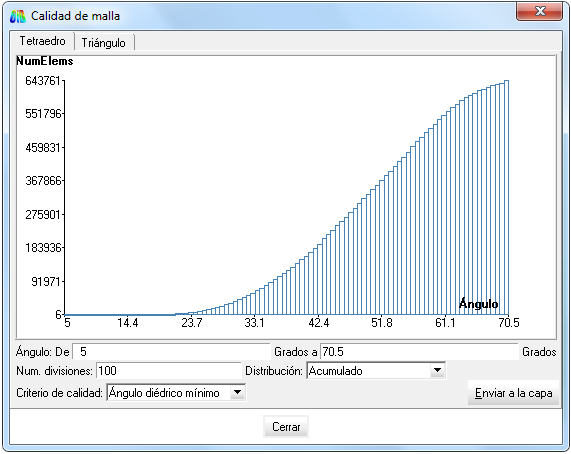
\includegraphics[scale=0.60]{img/cant_tetraedros}}
\caption{Calidad de la Malla - Tetraedros}
\label{calidadtetraedros}
\end{figure}

\begin{figure}[tbhp]
\centerline{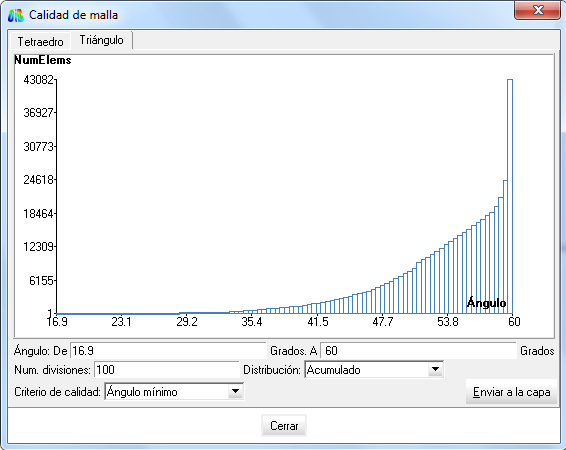
\includegraphics[scale=0.60]{img/cant_triangulos}}
\caption{Calida de la Malla - Triángulos}
\label{calidadtriangulos}
\end{figure}

\begin{figure}[tbhp]
\centerline{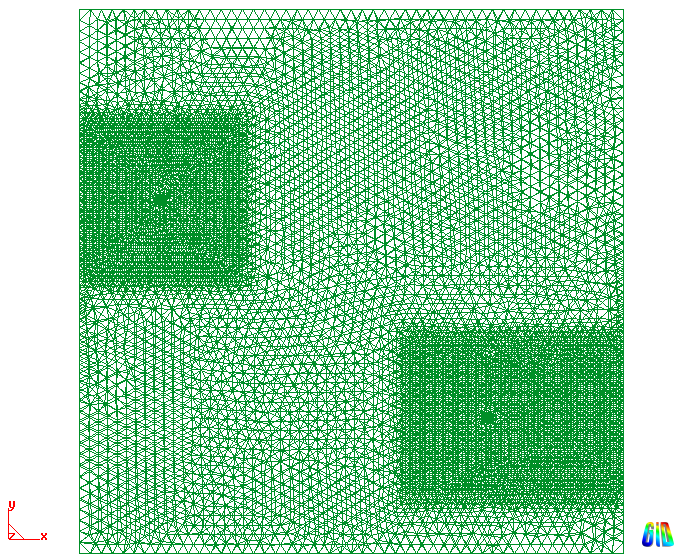
\includegraphics[scale=0.75]{img/contorno_malla_xy}}
\caption{Vista en el plano XY de la malla}
\label{contorno_malla_xy}
\end{figure}

%\begin{figure}[tbhp]
%\centerline{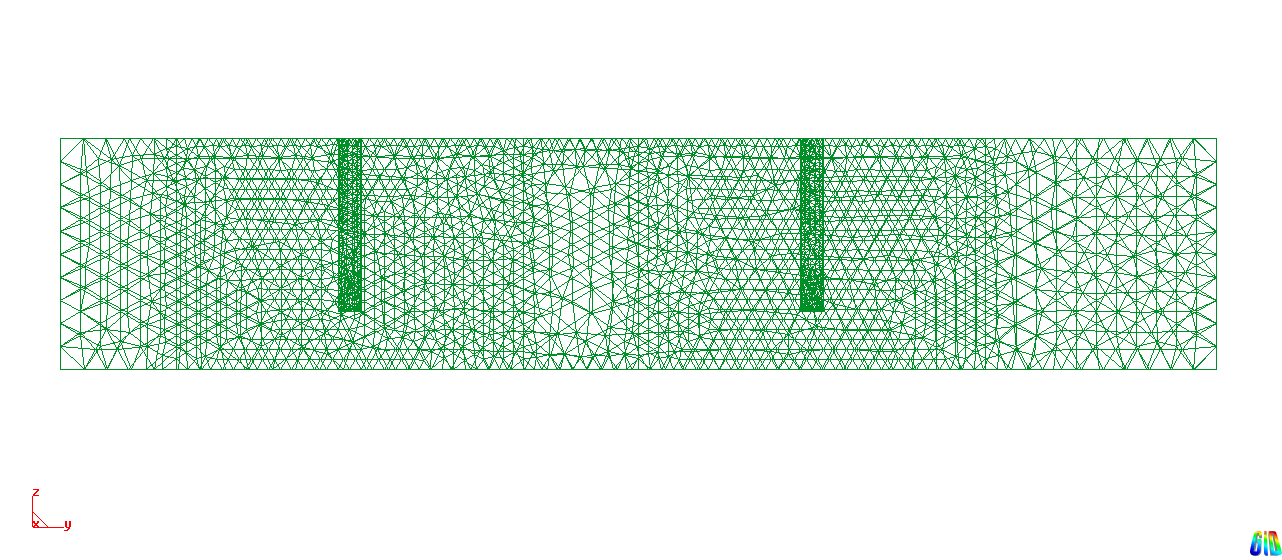
\includegraphics[scale=0.50]{img/contorno_malla_yz}}
%\caption{Vista en el plano YZ de la malla}
%\label{contorno_malla_yz}
%\end{figure}

\begin{figure}[tbhp]
\centerline{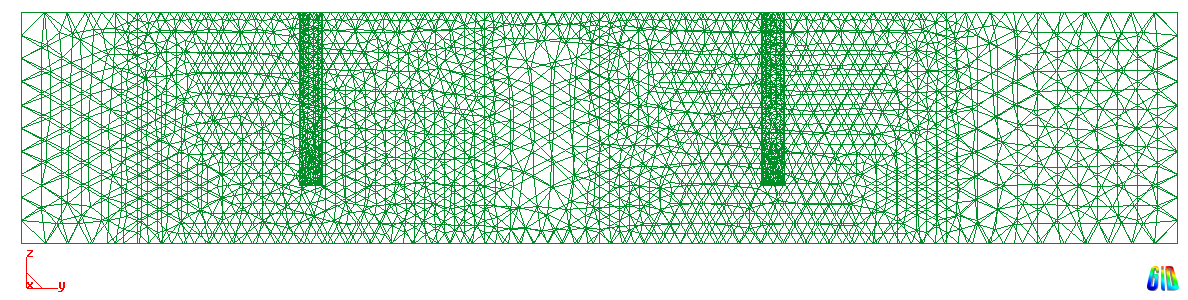
\includegraphics[scale=0.50]{img/contorno_malla_yz1}}
\caption{Vista en el plano YZ de la malla}
\label{contorno_malla_yz1}
\end{figure}

\begin{figure}[tbhp]
\centerline{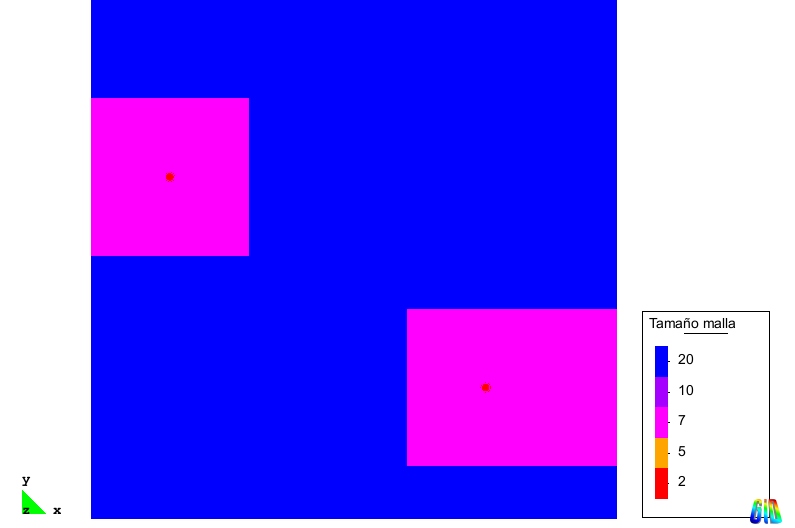
\includegraphics[scale=0.50]{img/tam_malla_xy}}
\caption{Tamaños de elementos de la malla - Vista en el plano XY}
\label{tam_malla_xy}
\end{figure}

\begin{figure}[tbhp]
\centerline{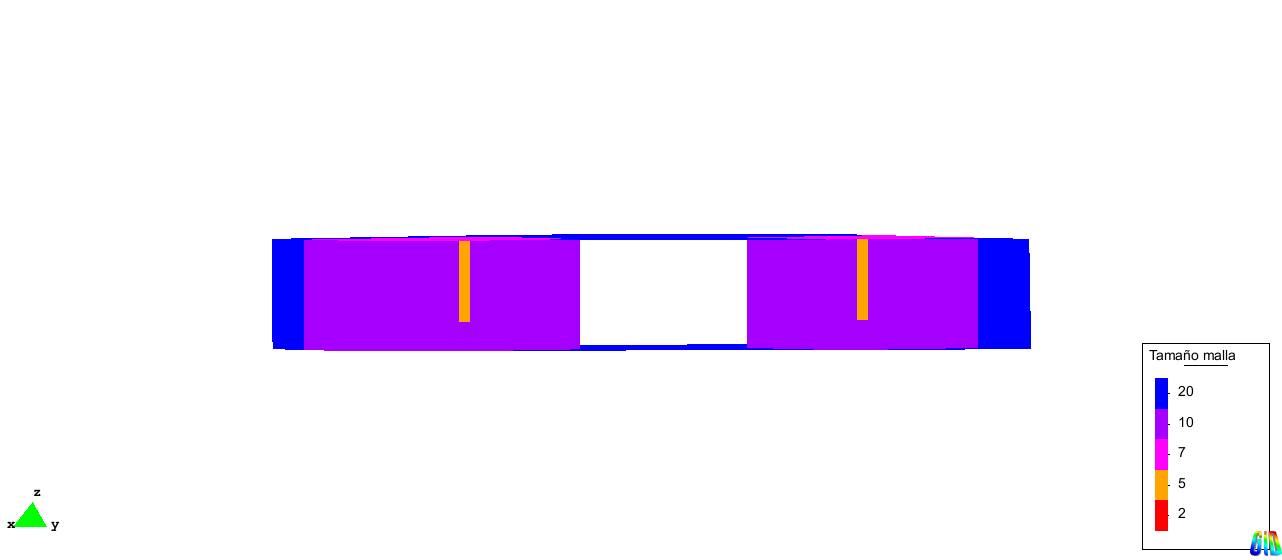
\includegraphics[scale=0.50]{img/tam_malla_pozo_interior}}
\caption{Tamaños de elementos de la malla - Corte transversal}
\label{tam_malla_pozo_interior}
\end{figure}
%%%%%%%%%%%%%%%%%%%%%%%%%%%%%%%%%%%%%%%%%%%%%%%%%%%%%%%%%%%%%%%%%%%%%%%%%%%%%%%%%%%%%%%%%%%%%%%%%%%
\subsection{Condiciones temporales}
describir como oelegimos en
%
%%%%%%%%%%%%%%%%%%%%%%%%%%%%%%%%%%%%%%%%%%%%%%%%%%%%%%%%%%%%%%%%%%%%%%%%%%%%%%%%%%%%%%%%%%%%%%%%%%%
\subsection{Ejecución}
cambiar el titulo esto es como se llevo a cabao la corrida

ver graficos en un nodo o punto la evolucion de una variable. -> point evolution ->velocity->module->elijo un nodo
%%%%%%%%%%%%%%%%%%%%%%%%%%%%%%%%%%%%%%%%%%%%%%%%%%%%%%%%%%%%%%%%%%%%%%%%%%%%%%%%%%%%%%%%%%%%%%%%%%
%%%%%%%%%%%%%%%%%%%%%%%%%%%%%%%%%%%%%%%%%%%%%%%%%%%%%%%%%%%%%%%%%%%%%%%%%%%%%%%%%%%%%%%%%%%%%%%%%%
%%%%%%%%%%%%%%%%%%%%%%%%%%%%%%%%%%%%%%%%%%%%%%%%%%%%%%%%%%%%%%%%%%%%%%%%%%%%%%%%%%%%%%%%%%%%%%%%%%
\section{Resultados}
v(veloc) -> lineas de flujo/vect
p->equipotenciales
realizar cortes

lo que vamos a ver va a ser las equipotenciales (lineas de presion que son perpendiculares al flujo).siempre es contraria a la linea de velocidad
%%%%%%%%%%%%%%%%%%%%%%%%%%%%%%%%%%%%%%%%%%%%%%%%%%%%%%%%%%%%%%%%%%%%%%%%%%%%%%%%%%%%%%%%%%%%%%%%%%
%%%%%%%%%%%%%%%%%%%%%%%%%%%%%%%%%%%%%%%%%%%%%%%%%%%%%%%%%%%%%%%%%%%%%%%%%%%%%%%%%%%%%%%%%%%%%%%%%%
%%%%%%%%%%%%%%%%%%%%%%%%%%%%%%%%%%%%%%%%%%%%%%%%%%%%%%%%%%%%%%%%%%%%%%%%%%%%%%%%%%%%%%%%%%%%%%%%%%
\section{Conclusiones}
si el mod respondio
que problemas tuvimos? ahi hacer mencion al pozo grande y tiempo de calculo...
pozo real vs pozo simulado
%%%%%%%%%%%%%%%%%%%%%%%%%%%%%%%%%%%%%%%%%%%%%%%%%
%%%%%%%%%%%%%%%%%%%%%%%%%%%%%%%%%%%%%%%%%%%%%%%%%
%%%%%%%%%%%%%%%%%%%%%%%%%%%%%%%%%%%%%%%%%%%%%%%%%
\end{document}